\section{Lucky Patcher} \label{section:luckypatcher-explain}
On its official website, Lucky Patcher is described as \grqq[...] a great Android tool to remove ads, modify apps permissions, backup and restore apps, bypass premium applications license verification, and more\grqq \cite{luckyPatcherOfficial}.
It is written by a developer calling himself ChelpuS and currently on version is 6.0.7 (03/03/2016).
\newline
Lucky Patcher offers different options to crack and alter applications.
It is not guaranteed that any of the options will succeed. \cite{luckyPatcherOfficial}
\newline
\gls{luckypatcherg} requires no technical knowledge and offers automatic cracking to non professionals.
This combination makes it a popular and an effective tool with a high potential for creating damage.
\newline
\begin{figure}[h]
    \centering
    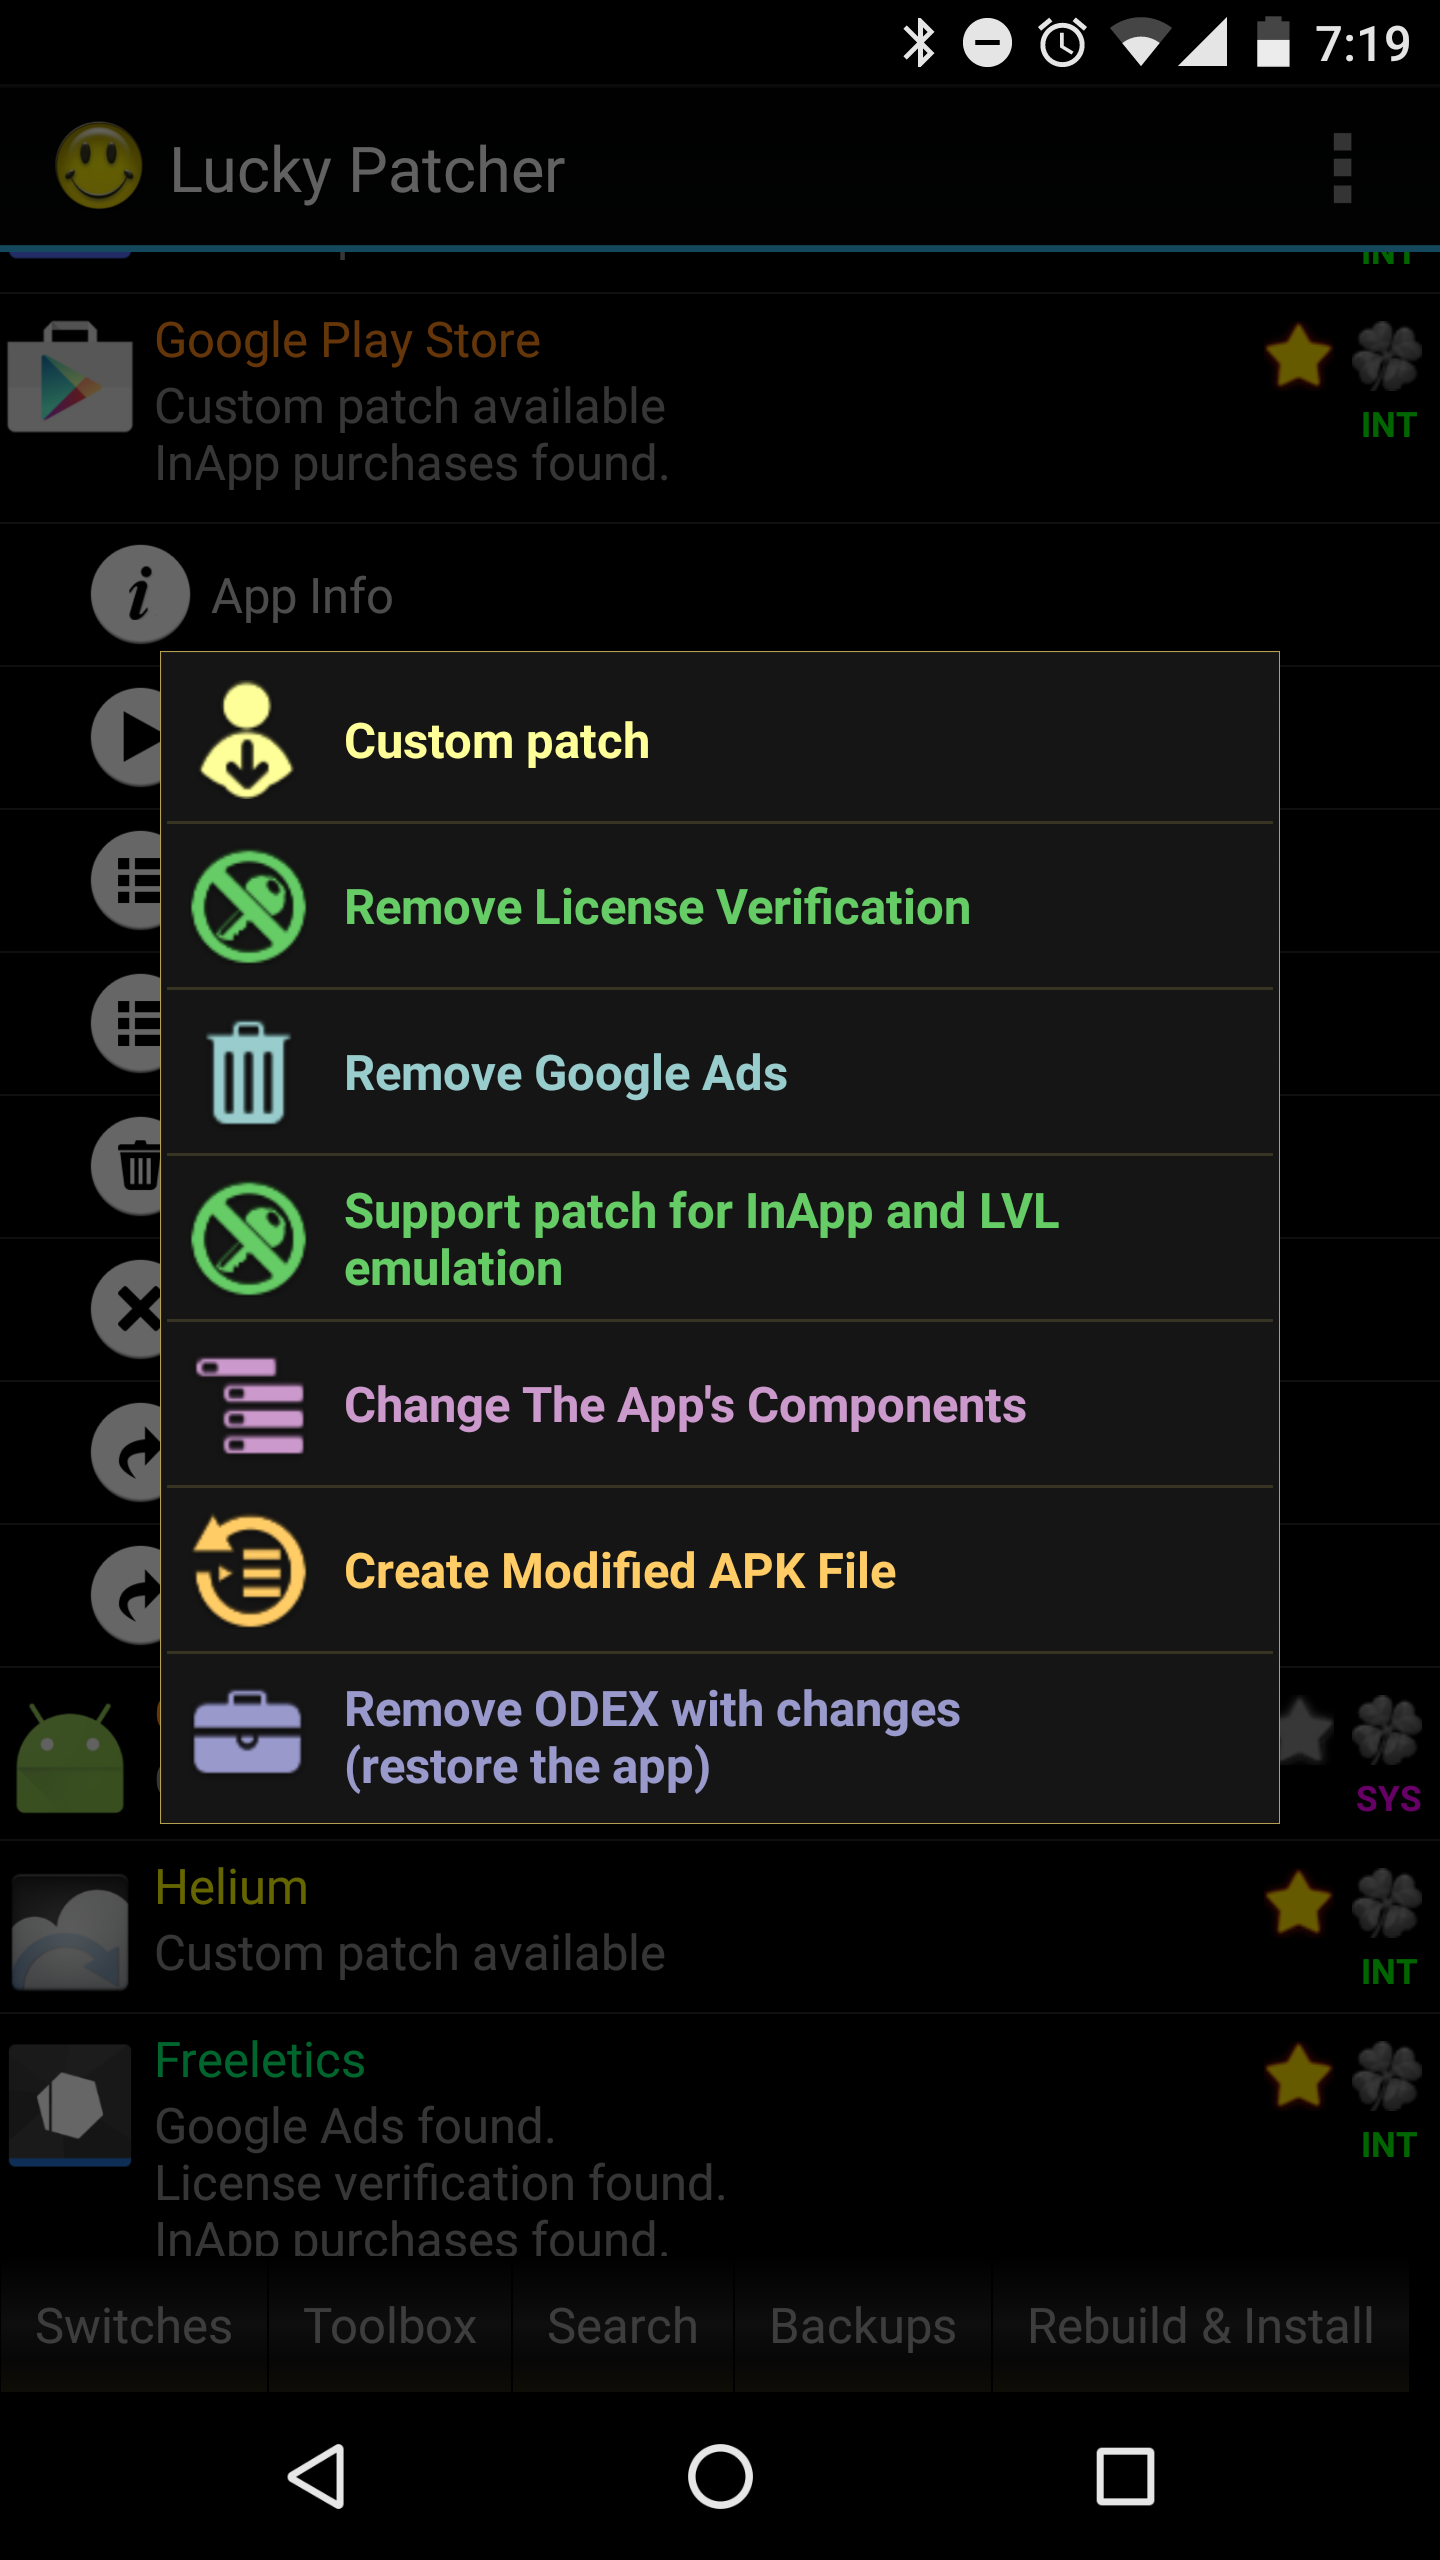
\includegraphics[width=0.3\textwidth]{data/luckyFeatures.png}
    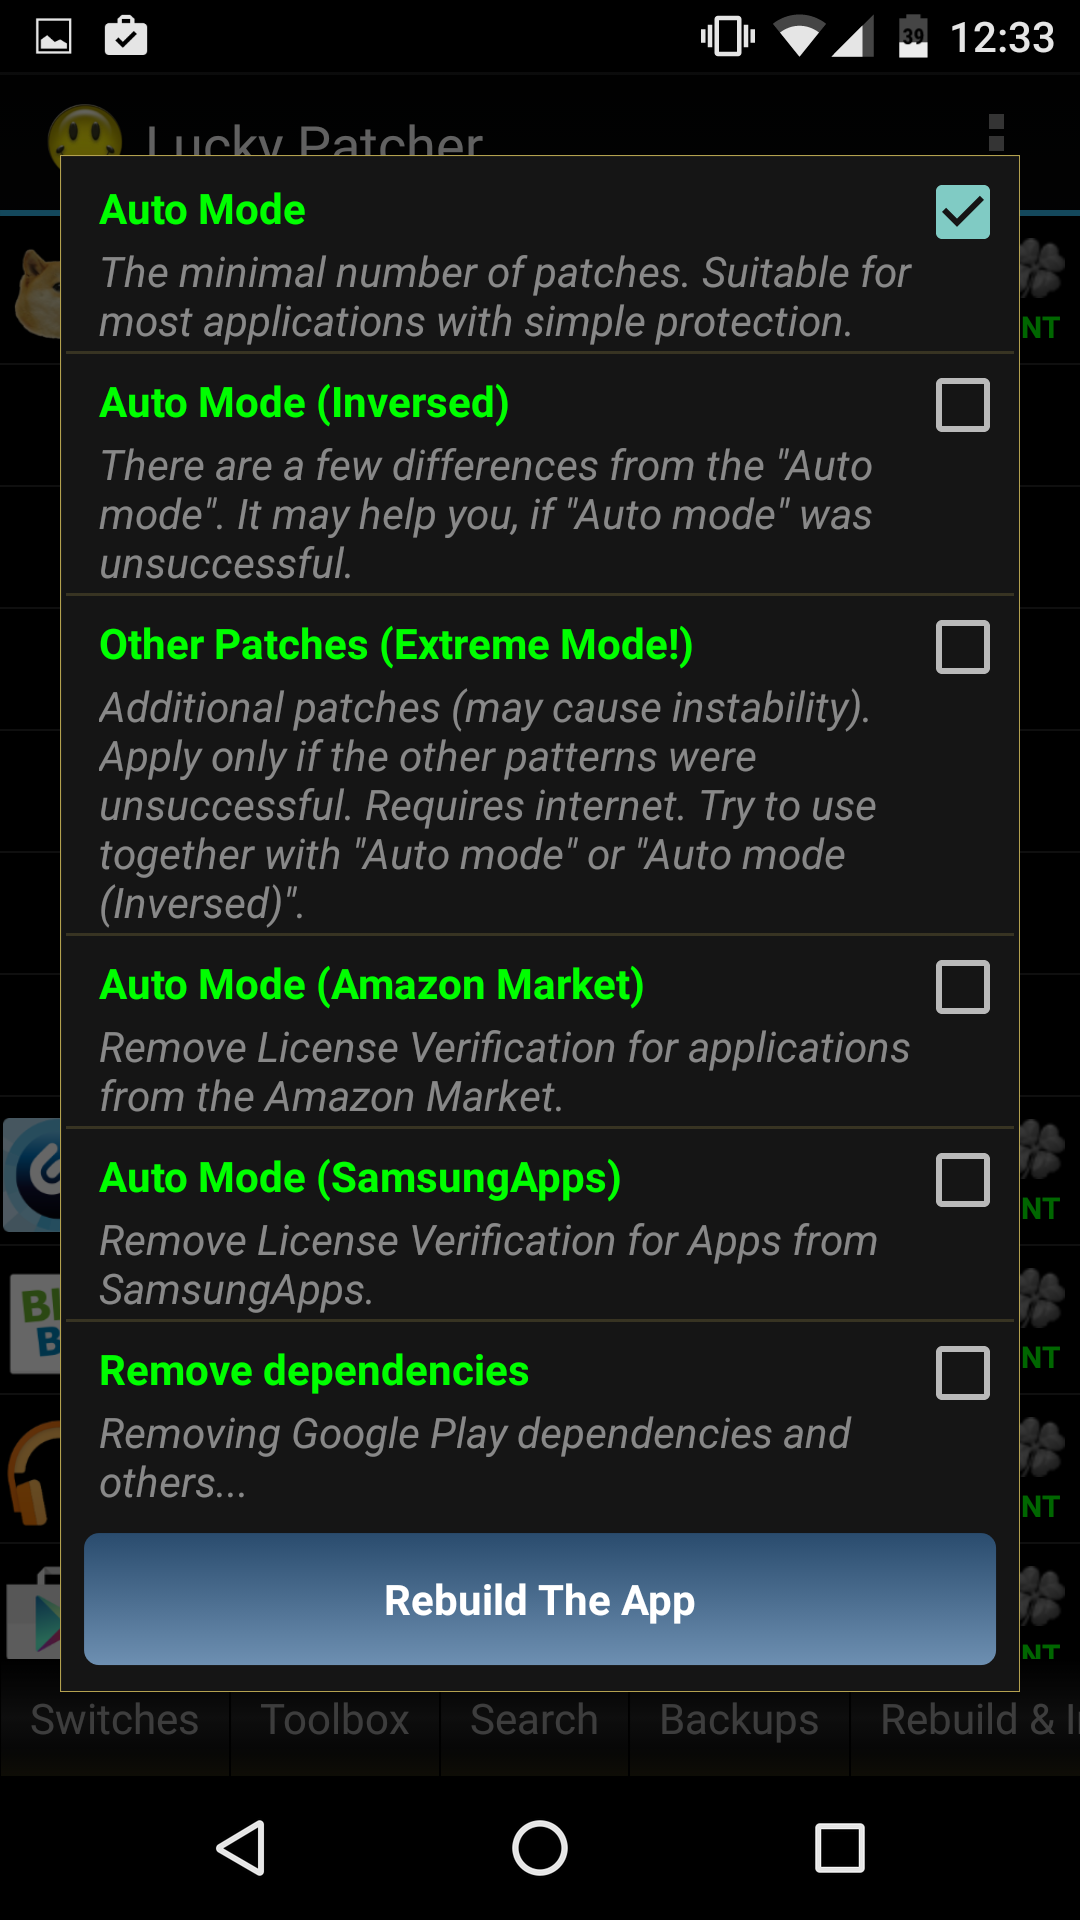
\includegraphics[width=0.3\textwidth]{data/luckyModi.png}
    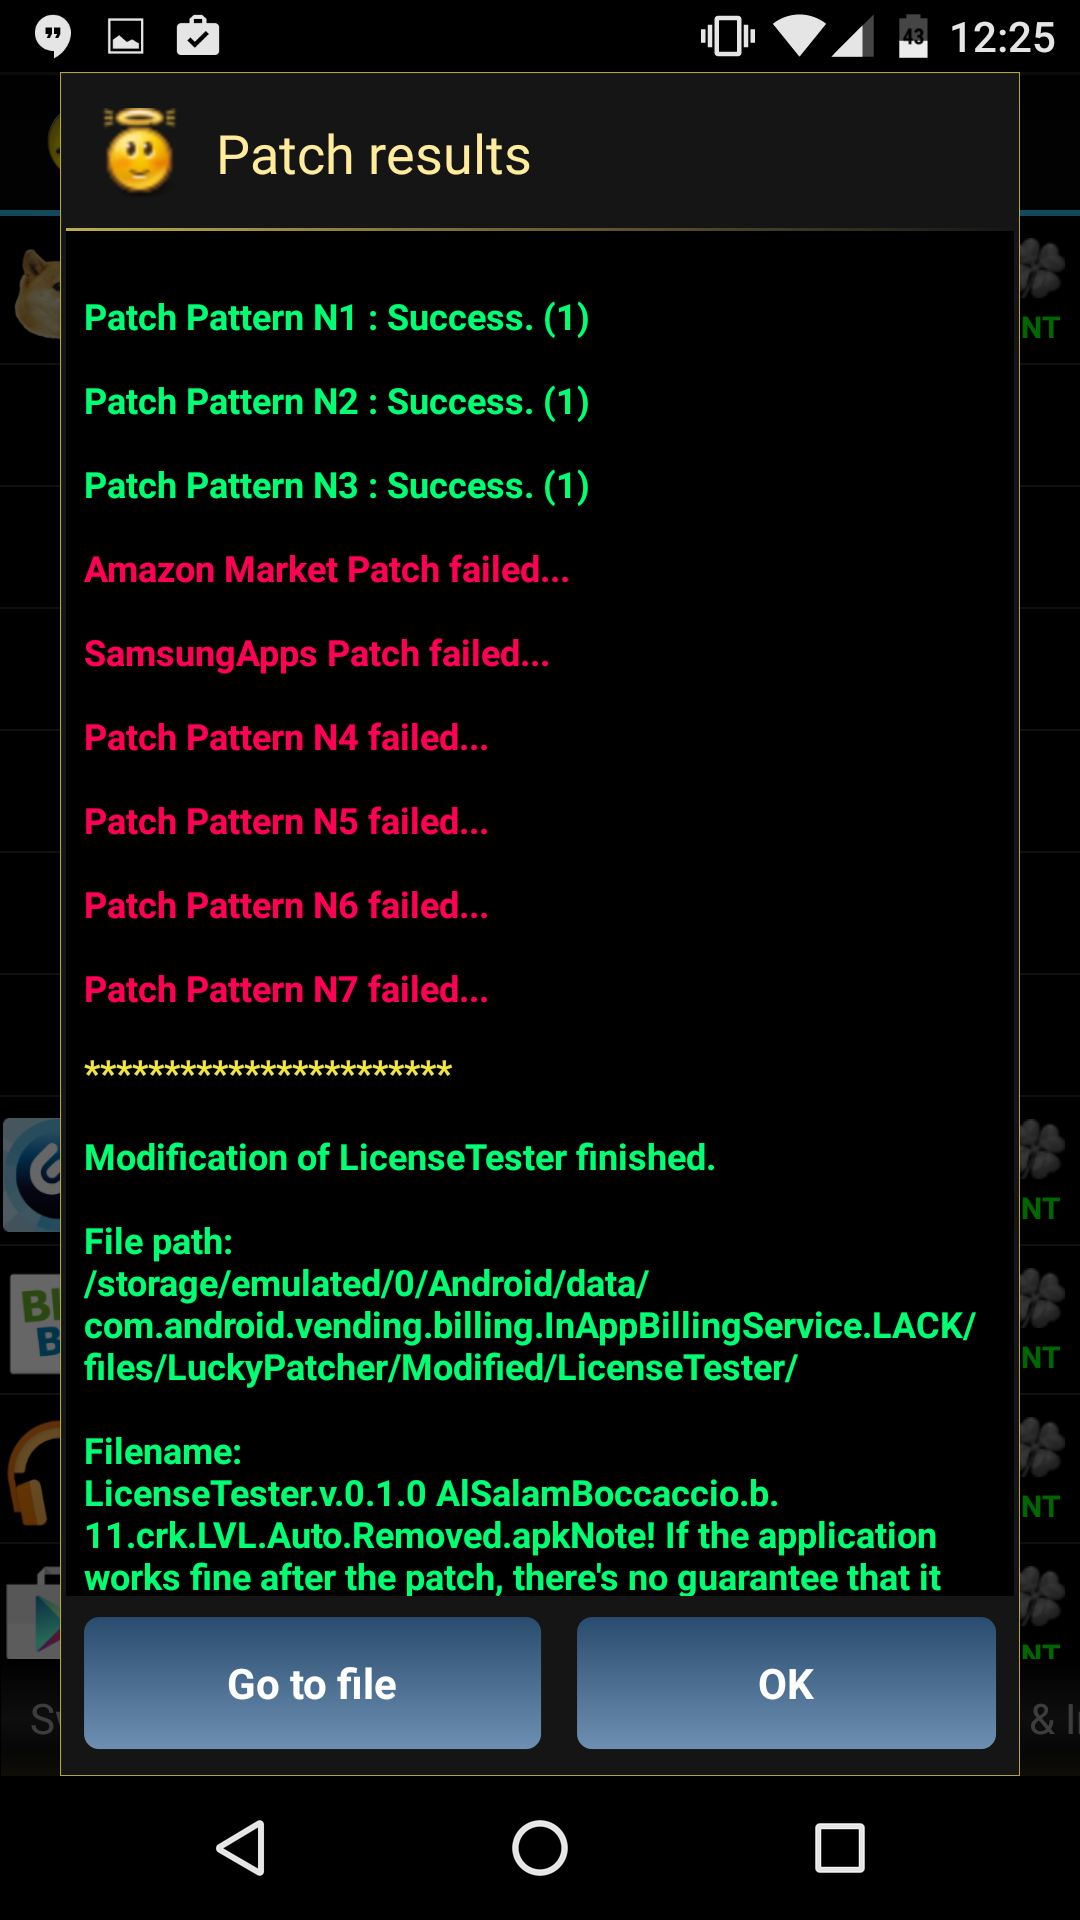
\includegraphics[width=0.3\textwidth]{data/luckyPatching.png}
    \caption{Left to right: Features offered LuckyPatcher, modes to crack license verification and the result after patching}
    \label{fig:luckyScreen}
\end{figure}
The application can be downloaded as an \gls{apk} from the official website \cite{luckyPatcherOfficial} and installed on any device, \textit{root} is not neccessarily required.
After the launch of \gls{luckypatcherg}, all installed applications are shown in a list.
A colored text indicates what patches are available and can be applied to an application.
Only when all features of \gls{luckypatcherg} are needed, the device has to be rooted \cite{luckyPatcherOfficial}.
\newline
When an application is selected, a submenu offers various actions, e.g. to get information about the app or run it.
The patches menu opens the submenu of figure~\ref{fig:luckyScreen}, on the left.
It shows the available patches for this application.
\newline
There are two types of patches.
The first type is the \textit{custom patch} and the second type are \textit{universal} patches.
The custom patch option applies changes specifically designed for a chosen application.
\newline
\textit{Universal} patches can be applied for the disabling of the license verification libraries, removal of Google Ads and rebuilding of the application to use the emulated \gls{lvl} and in-app billing \gls{api}.
\newline
\gls{luckypatcherg} offers two different approaches to apply these patches.
The first approach is to apply them directly on the device and requires \textit{root}.
This method creates an \gls{odex} version of the patched application in the Dalvik cache on the device.
The second approach is the creation of a modified \gls{apk}.
This approach extracts the application of choice from the storage, applies the selected modifications and creates a new \gls{apk}.
This cracked application can either be installed on the device after removing the original \gls{apk} or transferred to another device.
\newline
Both approaches offer the custom and \textit{universal} patches.
\newline
\newline
The focus in this thesis is on the \textit{universal} patches for removing of the license verification by creating a modified \gls{apk}.
\newline
There are five \textit{universal} modes and two \textit{universal} patches available for removing the license verification as seen in figure~\ref{fig:luckyScreen} in the middle.
Their description is rather short and does not offer information of how the modes are applied and working.
\newline
The patching starts when a mode is selected.
When the process is finished, a result screen is shown as seen in figure~\ref{fig:luckyScreen} on the right.
It indicates that different patches were applied.
